\section{Experimental Evaluation}
\label{sec:experimental_evaluation}

This section evaluates the effectiveness of vLLM-FI and the reliability of large language models under different fault conditions. We first describe the experimental setup and then calibrate the fault injection behavior of vLLM-FI against MRFI. We then analyze the effects of compute and memory faults across downstream tasks and evaluate how weight-only quantization affects sensitivity to memory faults. Finally, we examine reliability differences in distributed inference, including those associated with communication strategies and model-parallel configurations. Unless otherwise specified, the fault injection scope covers all model layers. For device-specific injection in model-parallel experiments, the scope covers all model layers or layer partitions assigned to the selected GPU.

\section{Experimental Setup}
\label{sec:experimental_setup}

This section reports the common setup used to validate vLLM-FI and evaluate LLM inference reliability.

\subsection{Experimental Platform and Workloads}
\label{subsec:platform_workloads}

Experiments run on a server with eight NVIDIA A100-SXM4-80GB GPUs. Distributed experiments use four GPUs. The software stack consists of Ubuntu 20.04.6, Python 3.12.11, PyTorch 2.6.0+cu124, CUDA 12.2, NCCL 2.21.5, vLLM 0.8.5 \cite{kwon2023efficient}, and \texttt{lm-evaluation-harness} 0.4.9.2. All tasks use fixed random seeds. Generative tasks disable sampling and use deterministic decoding.

LLaMA-3.1-8B \cite{grattafiori2024llama} is the primary model for tool validation, task-level reliability analysis, and quantization experiments.The quantization study evaluates AWQ W4A16 \cite{lin2024awq}, GPTQ W4A16, GPTQ W8A16 \cite{frantar2022gptq}, and FP8 W8A16 variants from the same model family. Communication and model-parallel experiments also include Qwen-2.5-7B \cite{yang2024qwen25} and Mistral-7B \cite{jiang2023mistral}.

The workload suite covers knowledge questions, commonsense reasoning, multidisciplinary knowledge, mathematical reasoning, text summarization, and code generation. ARC-Challenge, HellaSwag, MMLU, and GSM8K use the 100-sample configurations supplied by tinyBenchmarks \cite{polo2024tinybenchmarks} to control the cost of repeated fault-injection runs. Table~\ref{tab:workloads} lists the tasks and native metrics.

% This table is intentionally single-column and avoids resizebox/scalebox.
\begin{table}[t]
\caption{Downstream Workloads and Evaluation Metrics}
\label{tab:workloads}
\centering
\footnotesize
\renewcommand{\arraystretch}{1.10}
\setlength{\tabcolsep}{3.2pt}
\begin{tabularx}{\columnwidth}{@{}>{\raggedright\arraybackslash}X >{\centering\arraybackslash}p{0.43in} >{\centering\arraybackslash}p{0.38in} >{\raggedright\arraybackslash}p{0.78in}@{}}
\toprule
\textbf{Task} & \textbf{Samples} & \textbf{Shots} & \textbf{Metric} \\
\midrule
\multicolumn{4}{@{}l}{\itshape Multiple-choice tasks} \\
tinyARC \cite{clark2018think}              & 100   & 25 & Norm. accuracy \\
tinyHellaSwag \cite{zellers2019hellaswag} & 100   & 10 & Norm. accuracy \\
tinyMMLU \cite{hendrycks2020measuring}    & 100   & 0  & Norm. accuracy \\
\addlinespace[2pt]
\multicolumn{4}{@{}l}{\itshape Autoregressive generation tasks} \\
tinyGSM8K \cite{cobbe2021training}        & 100   & 5  & Exact Match \\
CNN/DailyMail \cite{hermann2015teaching}  & 1,149 & 0  & ROUGE-1 \cite{lin2004rouge} \\
HumanEval \cite{chen2021evaluating}       & 164   & 0  & Pass@1 \\
\bottomrule
\end{tabularx}
\end{table}

\subsection{Evaluation Protocol}
\label{subsec:evaluation_protocol}

The fault-free performance of each task and model configuration serves as its baseline. Let $m_{\mathrm{clean}}$ denote this baseline and $m_{\mathrm{fault}}^{(i)}$ the metric from fault-injection run $i$. Performance retention is
\begin{equation}
    R^{(i)}=\frac{m_{\mathrm{fault}}^{(i)}}{m_{\mathrm{clean}}}.
    \label{eq:performance_retention}
\end{equation}
A value of $R=1$ matches the fault-free baseline. A smaller value indicates greater degradation. Each quantized configuration uses its own fault-free result as the baseline.

Section~5 presents tool correctness and runtime cost, memory and compute faults across tasks, quantized representations, communication paths, and TP/PP rank selection. Each result subsection begins with its experiment-specific fault settings and controls, followed by quantitative results and analysis.


\subsection{Tool Validation and Calibration}
\begin{figure}[t]
    \centering
    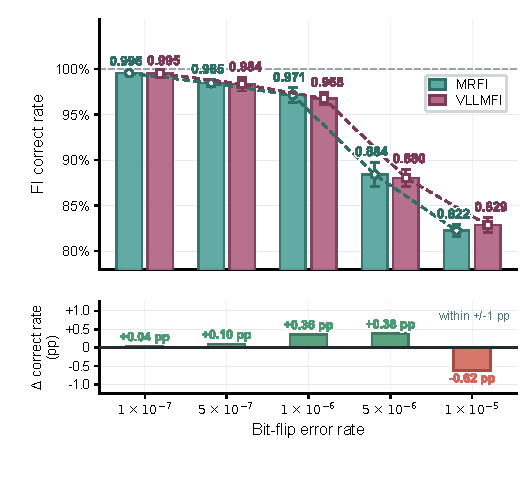
\includegraphics[width=\columnwidth]{fig_exp1_consistency_analysis.pdf}
    \caption{\textbf{Output-level consistency between MRFI and vLLM-FI.}
vLLM-FI closely matches MRFI across different bit flip error rates, showing highly consistent FI correct rates.}
    \label{fig:exp1_consistency_analysis}
\end{figure}

\begin{figure}[t]
    \centering
    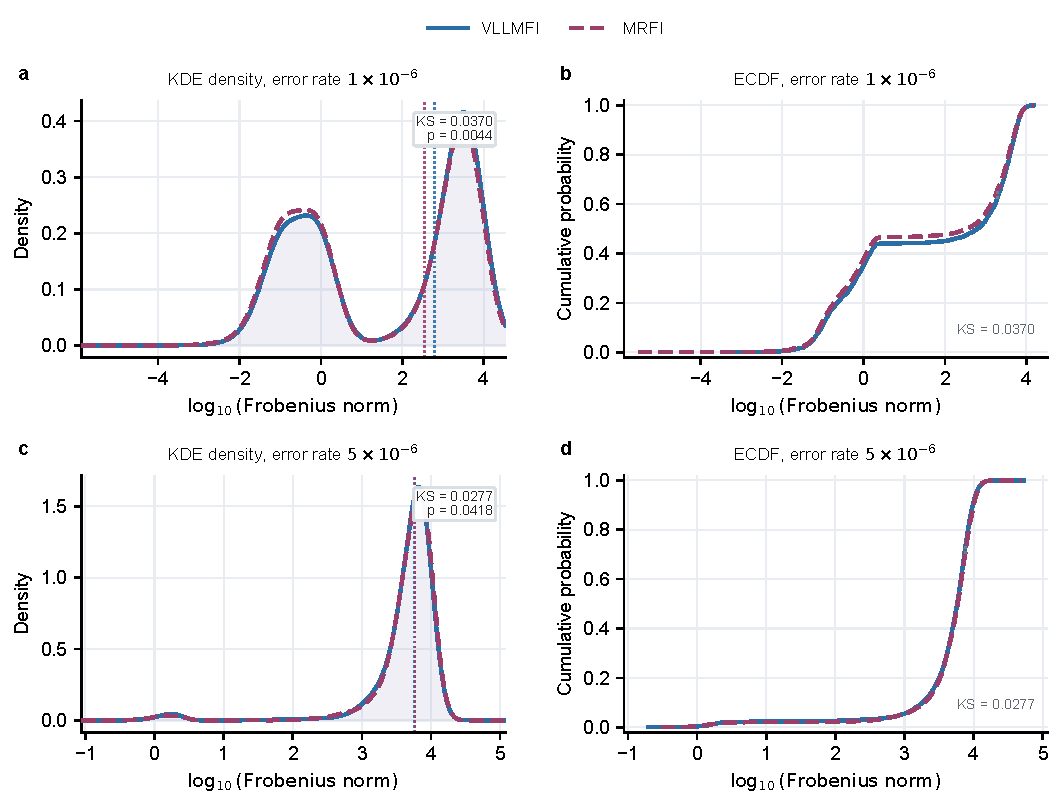
\includegraphics[width=\columnwidth]{fig_exp1_frob_distribution.pdf}
    \caption{\textbf{Tensor-level calibration against MRFI.}
    vLLM-FI produces activation perturbation distributions that closely match MRFI under different bit flip error rates.}
    \label{fig:exp1_frob_distribution}
\end{figure}

\textbf{Calibration Protocol.}
We calibrated vLLM-FI against MRFI at both the output and tensor levels. For each calibration setting, we performed five repetitions of 1,000 fault-injection trials on the same input sample. In both tools, all faults targeted the \texttt{down\_proj} module of the eighth model layer. For output-level analysis, we recorded whether the model produced the correct final output. For tensor-level analysis, we recorded the target-layer activations before and after fault injection.

\textbf{Output-Level Calibration.}
Figure~\ref{fig:exp1_consistency_analysis} compares the output-level fault effects produced by MRFI and vLLM-FI under different bit-flip error rates. The fault-injection (FI) correct rate is defined as the proportion of trials in which the model still produces the correct output after fault injection. Across all tested error rates, vLLM-FI closely matched MRFI, with a mean correlation coefficient of $r=0.999$ and a maximum absolute difference of only 0.62 percentage points. These results indicate that vLLM-FI reproduces the output-level fault effects of MRFI while operating on the native vLLM inference path.

\textbf{Tensor-Level Calibration.}
Agreement in final-output correctness does not necessarily imply that the two tools produce similar intermediate perturbations. We therefore compared the changes in the target-layer activation matrices before and after fault injection. Figure~\ref{fig:exp1_frob_distribution} presents the distributions of the Frobenius norms of the activation changes produced by MRFI and vLLM-FI. Panels (a) and (b) show the kernel density estimate (KDE) and empirical cumulative distribution function (ECDF) curves at a bit-flip error rate of $1\times10^{-6}$, whereas panels (c) and (d) show the corresponding results at $5\times10^{-6}$. At both error rates, the two tools produced highly overlapping distributions. The low Kolmogorov--Smirnov (KS) statistics further indicate close agreement between the distributions of their activation-change magnitudes.

Taken together, the output-level and tensor-level analyses show that, under the tested settings, vLLM-FI closely matches MRFI in both final-output correctness and the distribution of activation-change magnitudes. This agreement supports the use of vLLM-FI in the subsequent large-scale experiments.

\begin{figure}[t]
    \centering
    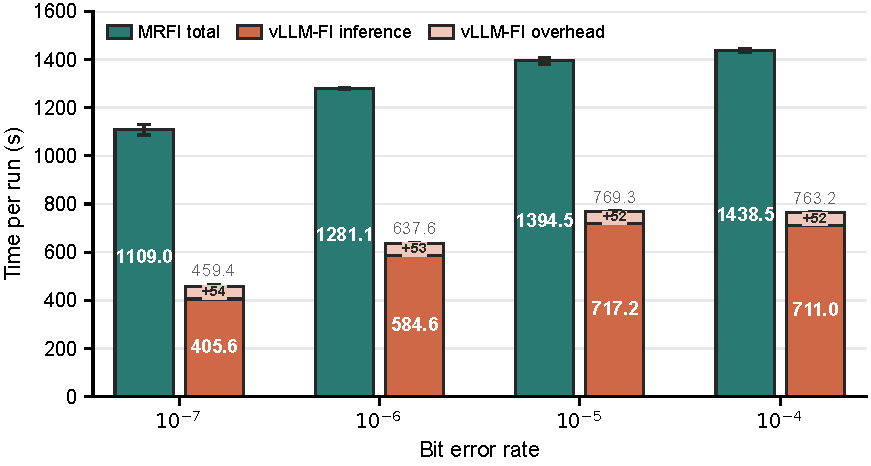
\includegraphics[width=\columnwidth]{exp1_mrfi_vllmfi_runtime_comparison.pdf}
\caption{\textbf{End-to-end runtime of MRFI and vLLM-FI.}
Bars show the mean runtime per run, with error bars denoting the standard deviation. The vLLM-FI runtime is divided into inference time and other runtime overhead.}
    \label{fig:mrfi_vllmfi_runtime}
\end{figure}

\textbf{End-to-End Runtime Comparison.}
We further compare the execution time of MRFI and vLLM-FI when faults are injected into all \texttt{down\_proj} modules in the model. The evaluated bit-flip error rates range from $10^{-7}$ to $10^{-4}$. Figure~\ref{fig:mrfi_vllmfi_runtime} reports the mean wall-clock time per run, with error bars indicating the sample standard deviation.

Across all tested error rates, vLLM-FI requires between $7.66$ and $12.82$ minutes per run, compared with $18.48$ to $23.98$ minutes for MRFI. This corresponds to a wall-clock time reduction of $44.8\%$--$58.6\%$, or a speedup of $1.81\times$--$2.41\times$. Model inference accounts for $88.3\%$--$93.2\%$ of the total vLLM-FI runtime, while the remaining runtime overhead remains nearly constant at approximately $52.1$--$53.8$ seconds. These results demonstrate that vLLM-FI reduces the end-to-end cost of repeated fault-injection experiments under the evaluated all-\texttt{down\_proj} injection workload.


\begin{figure}[t]
    \centering
    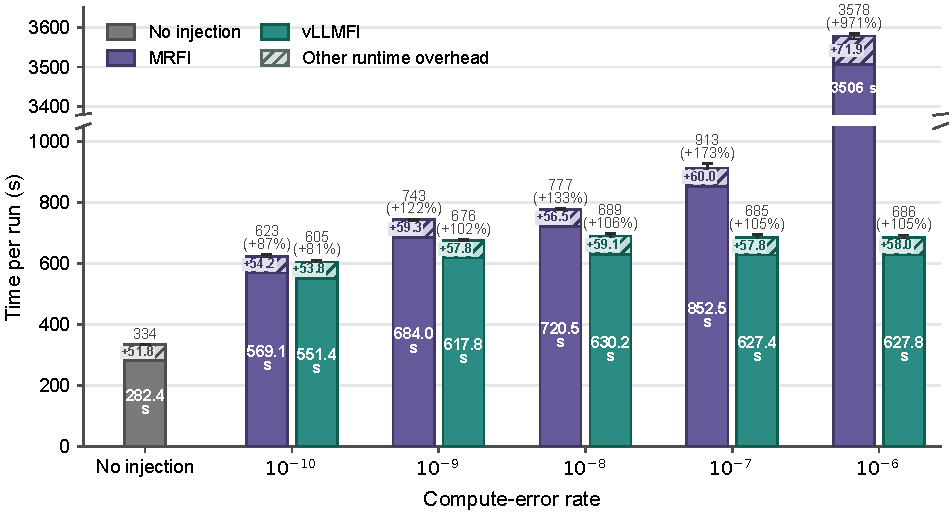
\includegraphics[width=\columnwidth]{extended_compute_error_runtime_comparison.pdf}
    \caption{\textbf{Controlled runtime comparison of MRFI-style and CUDA-based injection backends.}
    Mean runtime is reported for LLaMA-3.1-8B on GSM8K under compute-fault injection across all \texttt{down\_proj} modules. Percentages show increases over the no-injection baseline; the broken y-axis displays the MRFI-style result at $10^{-6}$.}
    \label{fig:controlled_injection_runtime}
\end{figure}

\textbf{Controlled Comparison of Injection Backends.}
To isolate the efficiency of the injection implementation from differences between inference frameworks, we ported the fault-injection logic of MRFI into the vLLM-FI runtime. We evaluate LLaMA-3.1-8B on GSM8K and inject compute faults into the outputs of all \texttt{down\_proj} modules. A fault-free execution is included as the baseline, and the evaluated compute-error rates range from $10^{-10}$ to $10^{-6}$.

Figure~\ref{fig:controlled_injection_runtime} shows that the runtime advantage of the CUDA backend increases with the error rate. At $10^{-10}$, the MRFI-style and CUDA backends require $623.3$ and $605.2$ seconds per run, respectively, corresponding to a modest reduction of $2.9\%$. As the error rate increases from $10^{-9}$ to $10^{-6}$, the runtime of the MRFI-style backend increases from $743.3$ to $3577.9$ seconds. In contrast, the CUDA backend remains between $675.6$ and $689.3$ seconds. At $10^{-6}$, the CUDA backend reduces wall-clock time by $80.8\%$ and achieves a $5.22\times$ speedup over the MRFI-style backend.

Taken together, the two runtime comparisons show that vLLM-FI reduces the end-to-end cost of repeated fault-injection experiments relative to MRFI and scales more efficiently as the fault rate increases. Under the evaluated workload targeting all \texttt{down\_proj} layers, the CUDA backend maintains comparatively stable runtime across the tested error rates, whereas the MRFI-style backend becomes substantially more expensive, yielding a maximum speedup of $5.22\times$ at $10^{-6}$. These results support the use of vLLM-FI for large-scale fault-injection campaigns.

\subsection{Reliability Assessment across Downstream Tasks}

\begin{figure}[t]
    \centering
    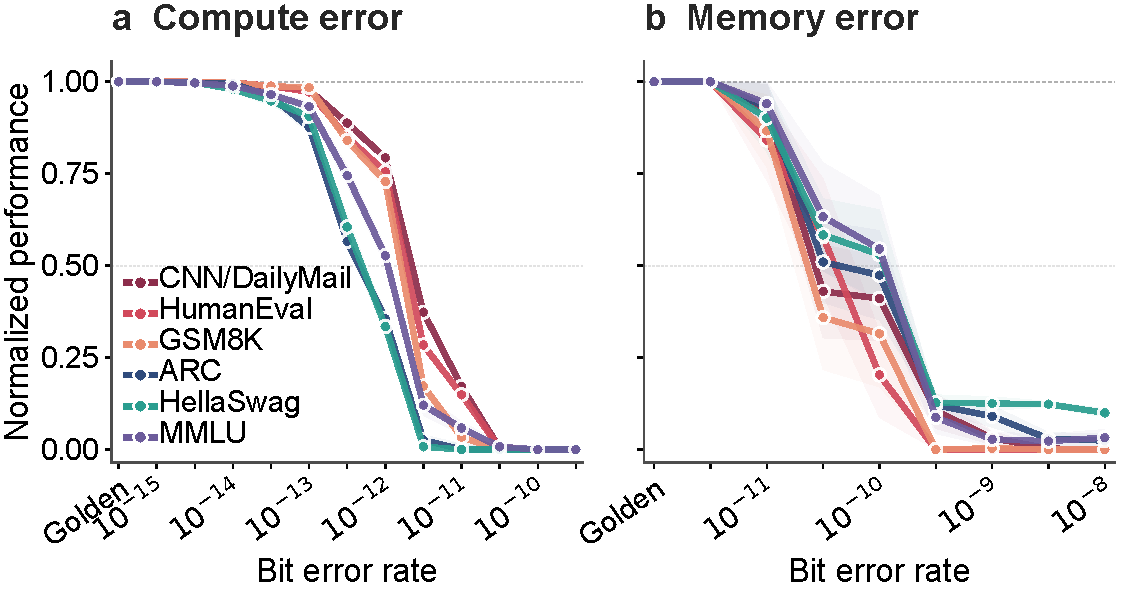
\includegraphics[width=\columnwidth]{fig_error_degradation_compute_memory.pdf}
    \caption{\textbf{Global degradation trends under compute and memory faults.}
    Compute and memory faults exhibit distinct reliability cliffs across downstream tasks.}
    \label{fig:error_degradation_compute_memory}
\end{figure}


\textbf{Global Degradation Trends.}
We characterize the reliability of Llama under compute and memory faults in two steps. The injection scope covers all layers of the Llama model, and multiple fault-injection runs are performed at each BER. We first scan a wide BER range over the full model to observe the global performance trajectory as the error rate increases. We then focus on the critical interval where the model transitions from near-baseline behavior to clear degradation and perform task-level evaluations within this interval.

Figure~\ref{fig:error_degradation_compute_memory} presents normalized task performance under compute and memory faults across downstream benchmarks. Both fault types exhibit localized reliability cliffs. The following task level analysis uses fault specific BER intervals selected from these global degradation trends.

\begin{figure}[t]
    \centering
    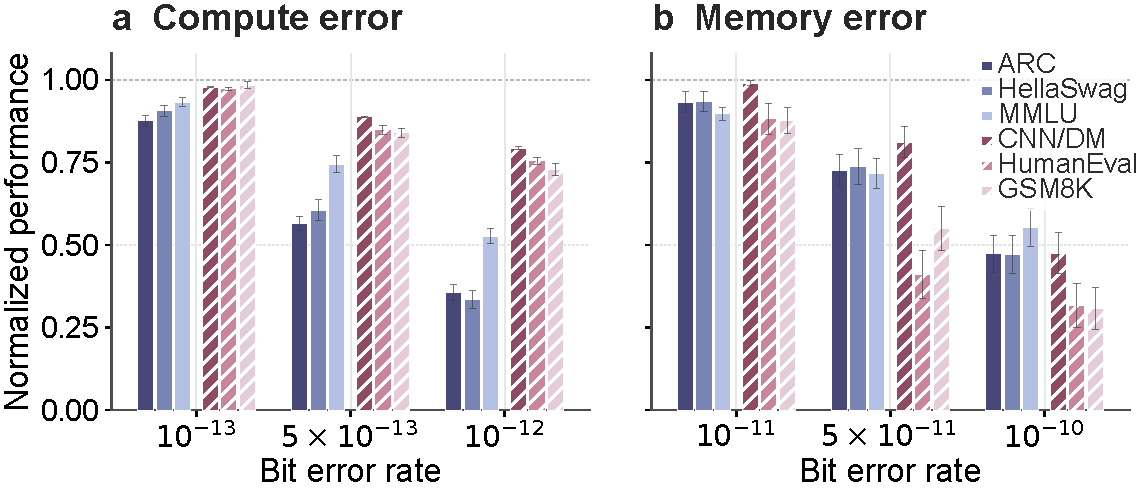
\includegraphics[width=\columnwidth]{fig_shadow_interval_task_performance.pdf}
    \caption{\textbf{Task level performance within critical BER intervals.}
    Compute and memory faults show opposite vulnerability patterns across multiple choice and generative tasks.}
    \label{fig:shadow_interval_task_performance}
\end{figure}


\textbf{Task Vulnerability Across Fault Models.} Figure~\ref{fig:shadow_interval_task_performance} presents task level performance within the critical BER intervals identified from the global degradation trends. Panel (a) shows normalized performance under compute faults from $10^{-13}$ to $10^{-12}$, while Panel (b) shows normalized performance under memory faults from $10^{-11}$ to $10^{-10}$. The evaluated benchmarks include three multiple choice tasks, ARC, HellaSwag, and MMLU, and three generative tasks, CNN/DailyMail, HumanEval, and GSM8K.

Restricting the analysis to the selected critical BER intervals reveals a fault-dependent reversal in task vulnerability, as summarized below.

\begin{observationbox}{Observation 1: Task vulnerability reverses across fault models}
Within the selected BER intervals, generative tasks are more vulnerable to memory faults, whereas multiple-choice tasks are more vulnerable to compute faults.
\end{observationbox}



This reversal can be explained by the different persistence and propagation behavior of the two fault models. Memory faults directly corrupt model weights, and their effects persist across subsequent layer computations. For generative tasks, such persistent perturbations can further affect intermediate states during auto regressive decoding, allowing errors to accumulate over multiple generation steps. In contrast, multiple choice tasks usually evaluate a fixed set of candidate answers and map model outputs to a discrete option space. Their final predictions are affected only when the perturbation changes candidate ranking or crosses a decision boundary.

Compute faults exhibit a different behavior because they are closer to local transient perturbations. A single activation perturbation usually affects a specific token or local output position, rather than persisting across subsequent inference steps as weight corruption does. For generative tasks, this local perturbation may be partially diluted by later contextual information, resulting in smoother performance degradation. For multiple choice tasks, however, the final answer often depends on key token representations and candidate logits. Local activation anomalies can therefore more directly change rankings near the decision boundary.


\begin{figure}[t]
    \centering
    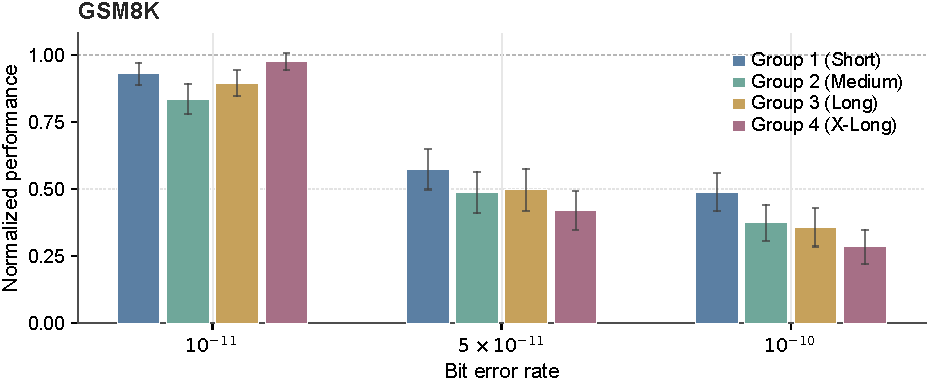
\includegraphics[width=\columnwidth]{fig_gsm8k_length_memory_error.pdf}
    \caption{\textbf{Effect of output length on GSM8K reliability under memory faults.}
    Longer generations show stronger degradation under persistent weight perturbations.}
    \label{fig:gsm8k_length_memory_error}
\end{figure}

\textbf{Effect of Generation Length.}
To further investigate why generative tasks are more sensitive to memory faults, we perform a sequence length ablation on GSM8K. GSM8K samples are first filtered to include only baseline correct examples. They are then grouped according to the token length of the model generated answer, measured by the Llama 3.1 8B tokenizer. Based on this length, the samples are divided into four groups: Short, Medium, Long, and X Long. Each group is evaluated under the same memory fault setting within the critical BER interval from $10^{-11}$ to $10^{-10}$.

As shown in Figure~\ref{fig:gsm8k_length_memory_error}, short output groups maintain higher normalized performance across the tested BER range, whereas longer output groups degrade more rapidly. This trend supports the interpretation that persistent weight perturbations can accumulate through repeated auto regressive decoding. Short sequence tasks may complete generation before the accumulated error becomes severe, whereas long sequence tasks undergo more decoding steps and are therefore more exposed to the persistent effects of memory faults.

\begin{observationbox}{Observation 2: Longer generation increases vulnerability to memory faults}
Under memory faults, GSM8K samples with longer target outputs exhibit more pronounced performance degradation. This indicates that the vulnerability of generative tasks is positively associated with the number of auto regressive decoding steps.
\end{observationbox}


\subsection{Reliability Assessment of Quantization Methods}

This section focuses on weight quantization, which is widely used in LLM deployment because it reduces memory footprint and bandwidth pressure.

\begin{figure}[t]
    \centering
    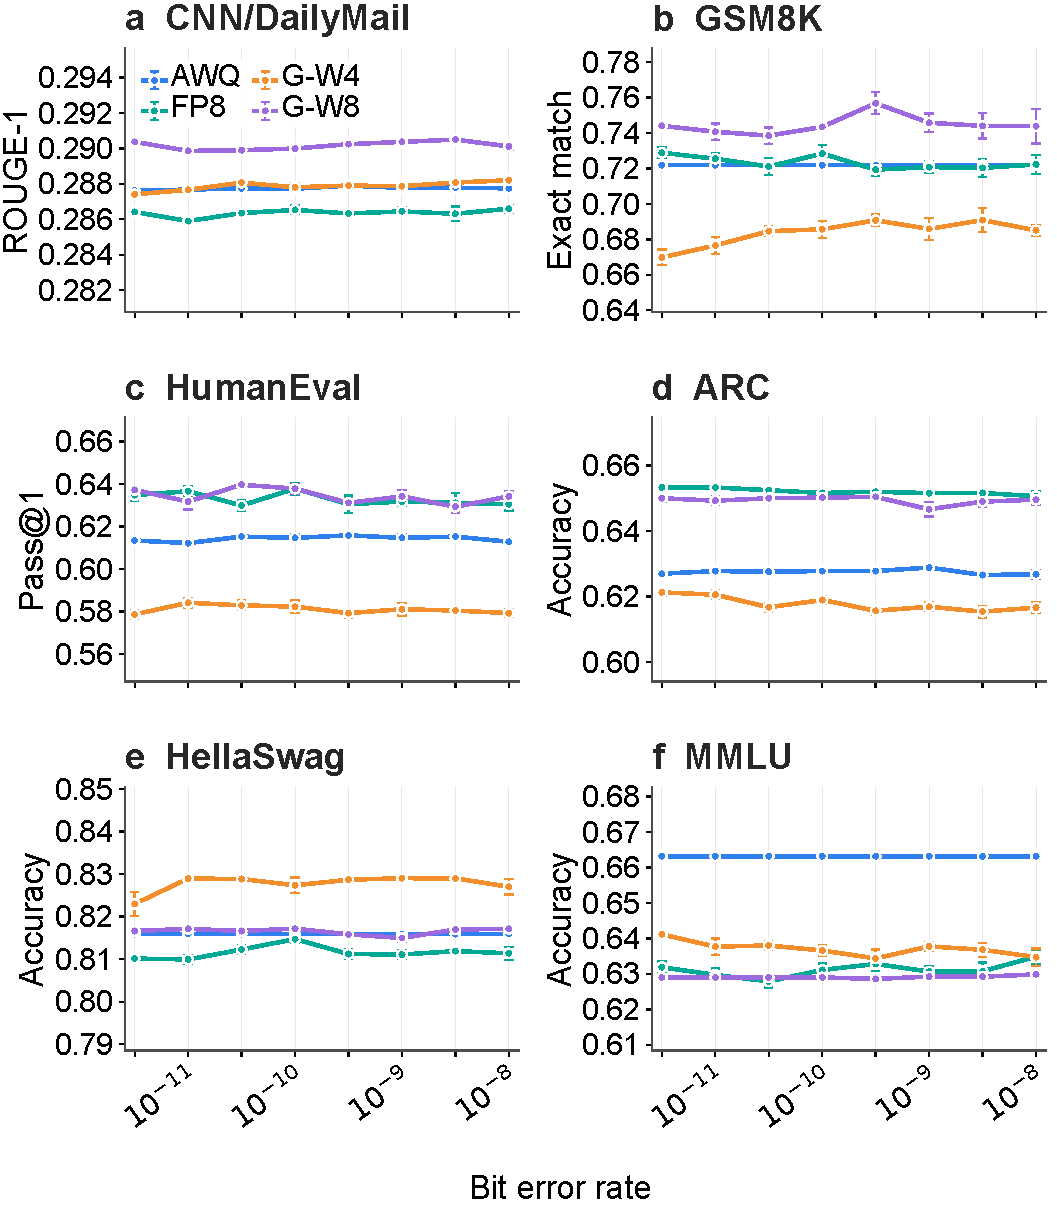
\includegraphics[width=\columnwidth]{fig_quantization_memory_error.pdf}
    \caption{\textbf{Reliability of weight quantized models under memory faults.}
    Quantized weight representations show relatively stable performance across downstream tasks.}
    \label{fig:quantization_memory_error}
\end{figure}

Figure~\ref{fig:quantization_memory_error} compares FP8, AWQ, GPTQ W4, and GPTQ W8 under memory faults across six downstream tasks. As in the preceding experiments, the fault-injection scope covers all model layers for each quantization configuration. The evaluated BER range spans from $5\times10^{-12}$ to $10^{-8}$. Across this range, weight-only quantized models show relatively stable performance, with no sharp degradation trend across the tested tasks.

\begin{observation}
\textbf{Observation 3:} Within the BER range evaluated in this study, weight  quantized models show relatively stable performance under memory faults, with no sharp degradation trend across the tested downstream tasks.
\end{observation}


This behavior may partly arise from the bounded representations used by quantized weights. Although INT4, INT8, and FP8 use different numerical encodings, their stored values are mapped to computation values through scaling or format conversion. For finite corrupted values, these representation ranges can limit the magnitude of resulting perturbations compared with FP16 or BF16, whose exponent-bit flips may produce much larger outliers or non-finite values.


Therefore, under memory faults, weight quantization may reduce the amplification of weight corruption by acting as an implicit numerical range constraint.


\subsection{Reliability Assessment under Different Communication Strategies}

This section investigates how communication-related faults affect model reliability during distributed inference. Unlike local computation faults, communication faults can propagate through cross-rank aggregation or inter-stage activation transfers. Consequently, their end-to-end effects may vary with the bit error rate (BER), communication frequency, synchronization scope, and fault propagation path of each parallelization strategy. To characterize these strategy-level differences, we compare tensor parallelism and pipeline parallelism under their native communication workloads.


\begin{figure}[t]
    \centering
    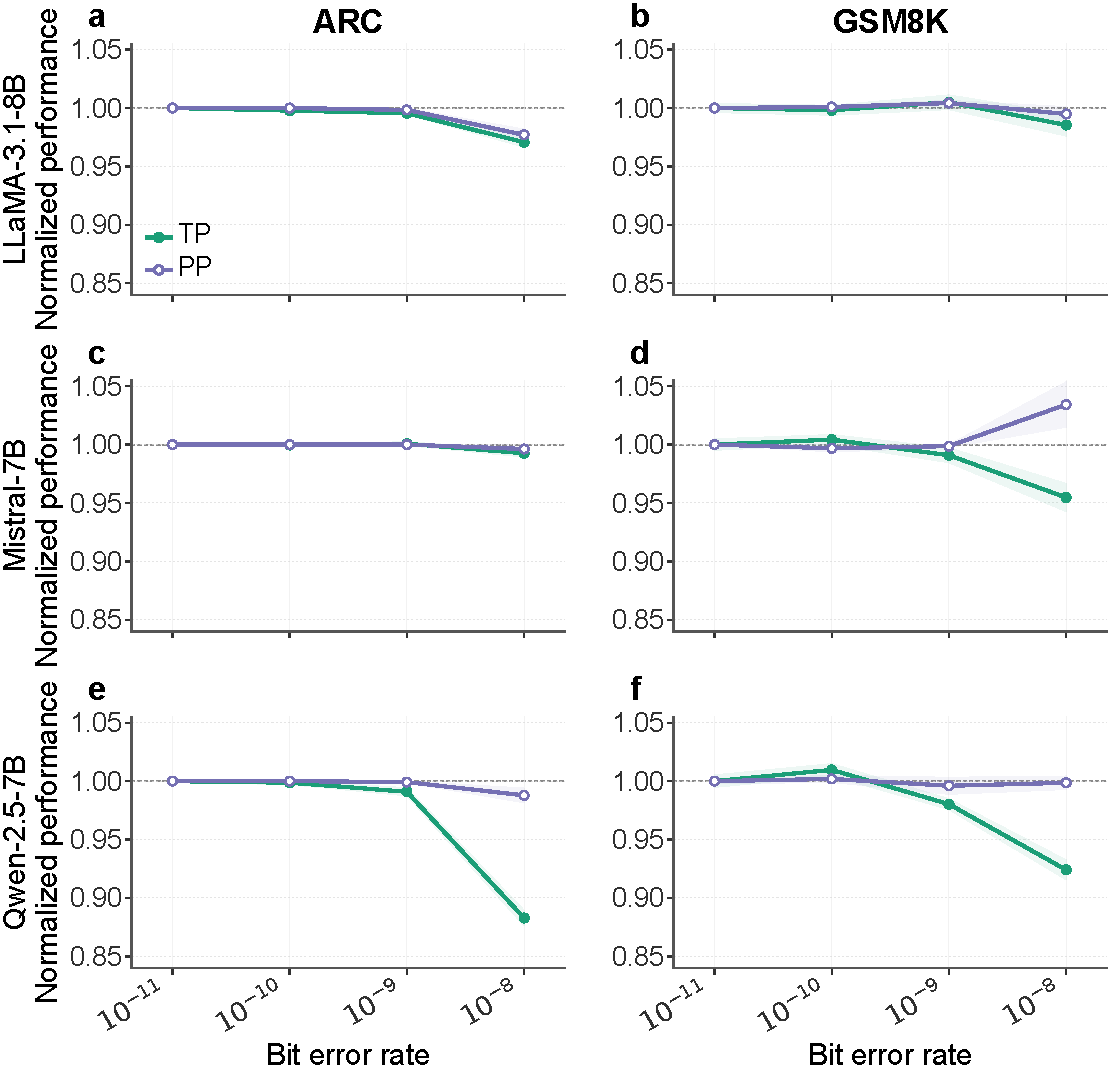
\includegraphics[width=\columnwidth]{fig_exp5_tp_pp_reliability_3x2_linechart.pdf}
    \caption{\textbf{End-to-end reliability of tensor parallelism and pipeline parallelism under communication-related faults.}
    Normalized performance is reported for LLaMA-3.1-8B, Mistral-7B, and Qwen-2.5-7B on ARC and GSM8K at BER points evaluated for both strategies. Solid blue lines denote tensor parallelism, whereas dashed orange lines denote pipeline parallelism.}
    \label{fig:tp_pp_communication}
\end{figure}

Figure~\ref{fig:tp_pp_communication} compares the performance degradation of tensor parallelism and pipeline parallelism under communication-related faults. To ensure a consistent horizontal comparison, we report only the BER values evaluated for both strategies. At the highest shared BER of $10^{-8}$, tensor parallelism and pipeline parallelism achieved mean normalized performances of $0.952$ and $0.998$, respectively. This result corresponds to an average advantage of $4.64$ percentage points for pipeline parallelism. Across individual tasks, pipeline parallelism exceeded tensor parallelism by $3.83$ percentage points on ARC and $5.45$ percentage points on GSM8K. The largest gap occurred for Qwen-2.5-7B on ARC, where tensor parallelism and pipeline parallelism achieved normalized performances of $0.883$ and $0.988$, respectively, corresponding to a difference of $10.50$ percentage points.

\begin{observation}
\textbf{Observation 4:} Within the evaluated BER range and native communication workloads, pipeline parallelism exhibits higher end-to-end reliability than tensor parallelism.
\end{observation}

The observed reliability gap may arise from the distinct communication patterns of the two strategies. Tensor parallelism invokes collective operations within multiple Transformer layers. At the same per-bit error rate, its higher communication frequency exposes more transmitted values to corruption, while cross-rank aggregation may spread corrupted values across multiple ranks. By contrast, pipeline parallelism mainly transfers activations between adjacent stages, so communication is concentrated at stage boundaries and faults primarily affect downstream stages.

These results characterize the end-to-end reliability of each parallelization strategy under its native communication workload. The normalized performance slightly above \(1.0\) for Mistral-7B on GSM8K under pipeline parallelism reflects run-to-run variation relative to the fault-free baseline and does not indicate a fault-induced performance gain.


% This section investigates how communication-related faults affect model reliability during distributed inference. Unlike faults in local computation, communication faults can propagate through cross-rank aggregation or inter-stage activation transfers. Their effects therefore depend not only on the bit error rate, but also on the communication frequency, synchronization scope, and fault propagation path associated with each parallelization strategy. We conduct two comparative experiments. First, we examine whether tensor parallelism introduces additional reliability risks relative to a baseline configuration without tensor parallelism. Second, we compare the degradation behavior of tensor parallelism and pipeline parallelism under communication-related faults.


% \begin{figure}[t]
%     \centering
%     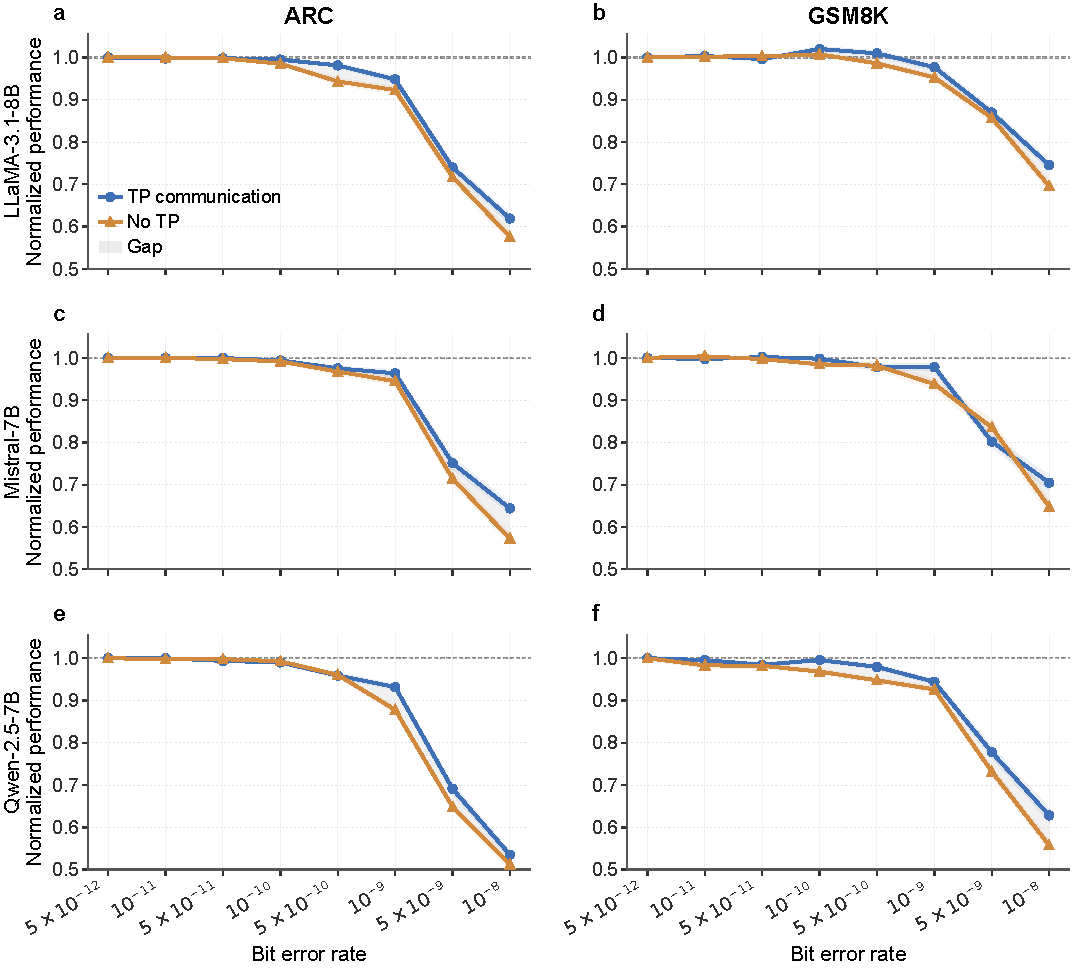
\includegraphics[width=\columnwidth]{fig_exp5_tp_no_tp_downproj_gap.pdf}
%     \caption{\textbf{Effect of tensor-parallel communication on fault sensitivity.}
%     Normalized performance of LLaMA-3.1-8B, Mistral-7B, and Qwen-2.5-7B on ARC and GSM8K under fault injection at the \texttt{down\_proj} layer. Blue curves denote the tensor-parallel communication setting, orange curves denote the setting without tensor parallelism, and shaded regions indicate the performance gap.}
%     \label{fig:tp_no_tp_communication}
% \end{figure}

% Figure~\ref{fig:tp_no_tp_communication} compares the reliability of tensor parallelism with that of the baseline configuration without tensor parallelism when faults are injected at the \texttt{down\_proj} layer. At low bit error rates, both configurations maintain normalized task performance close to $1.0$. As the bit error rate increases, both configurations exhibit noticeable degradation. Nevertheless, tensor parallelism preserves higher normalized performance across most model--task combinations.

% At the highest tested bit error rate of $10^{-8}$, tensor parallelism achieves an average normalized performance of $0.599$ on ARC, compared with $0.553$ for the baseline configuration. On GSM8K, the corresponding values are $0.693$ and $0.634$, respectively. The largest difference is observed for Mistral-7B on ARC, where tensor parallelism retains a normalized performance of $0.644$, whereas the baseline configuration achieves $0.572$, corresponding to a difference of $7.14$ percentage points.

% \begin{observation}
% \textbf{Observation 4:} Under the evaluated \texttt{down\_proj} injection setting and bit error rate range, tensor parallelism exhibits stronger fault tolerance than the baseline configuration without tensor parallelism.
% \end{observation}

% This behavior may be associated with the partial-result aggregation used by the tensor-parallel implementation of \texttt{down\_proj}. In the row-parallel configuration considered in this study, each rank computes a partial projection result, after which the partial results are aggregated through collective communication. A fault injected before this aggregation initially perturbs only the local contribution produced by one rank, which is subsequently combined with the contributions from the remaining ranks. By contrast, in the baseline configuration without tensor parallelism, the injected fault directly perturbs the complete projection result.

% Because partial and complete tensors can differ in their numerical distributions and dynamic ranges, an identical bit flip does not necessarily induce a perturbation of the same numerical magnitude in the two configurations. This difference provides a plausible explanation for the higher reliability observed with tensor parallelism. However, the effect may depend on the injection location, tensor-parallel degree, numerical format, and communication implementation, and should therefore not be generalized to all tensor-parallel configurations.



% \begin{figure}[t]
%     \centering
%     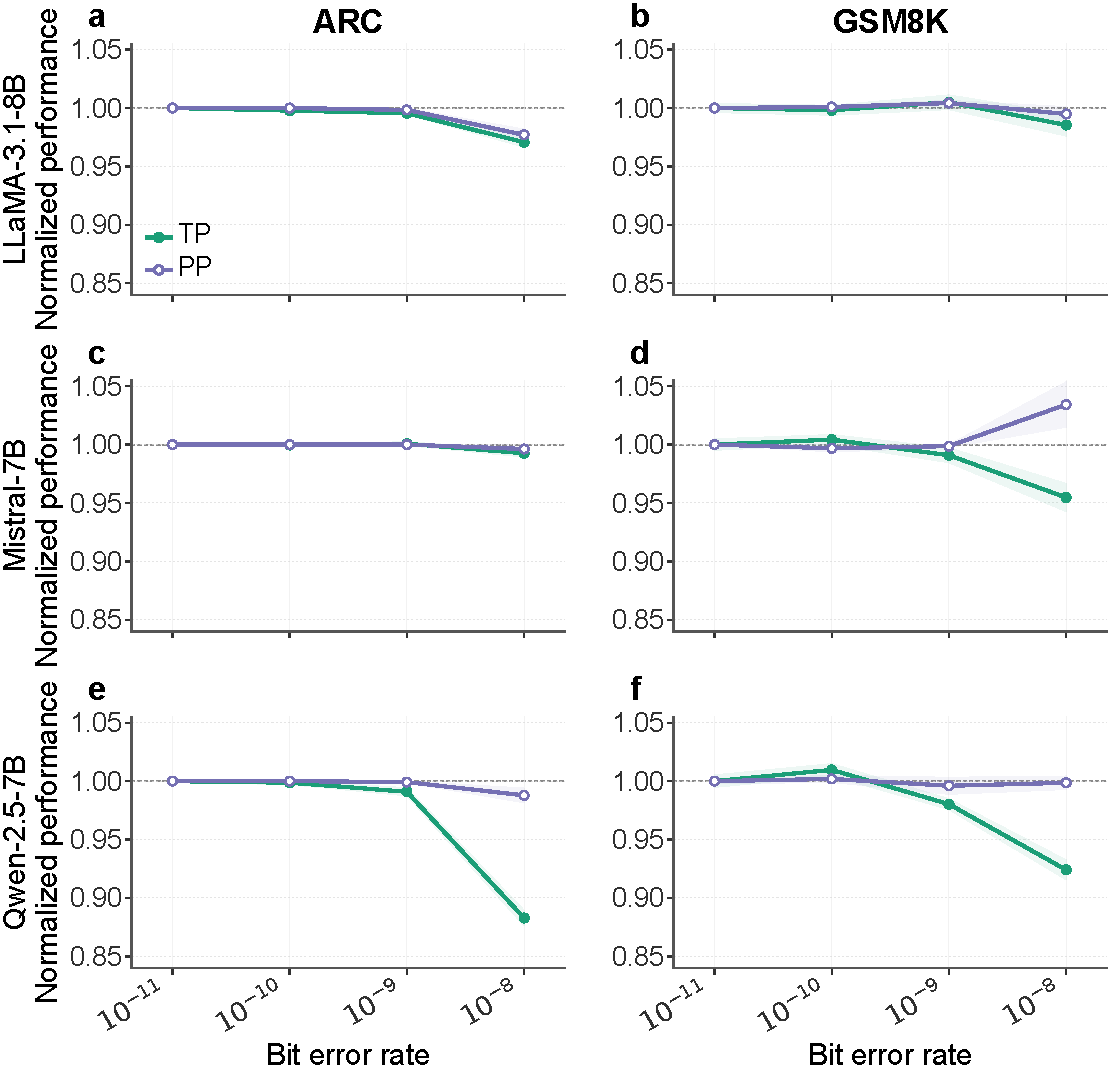
\includegraphics[width=\columnwidth]{fig_exp5_tp_pp_reliability_3x2_linechart.pdf}
%     \caption{\textbf{Reliability comparison between tensor parallelism and pipeline parallelism under communication related faults.}
%     Normalized performance is reported for LLaMA-3.1-8B, Mistral-7B, and Qwen-2.5-7B on ARC and GSM8K using shared BER points. Solid blue lines denote tensor parallelism, and dashed orange lines denote pipeline parallelism.}
%     \label{fig:tp_pp_communication}
% \end{figure}

% Figure~\ref{fig:tp_pp_communication} further compares tensor parallelism and pipeline parallelism under communication-related faults. To ensure a consistent horizontal comparison, the figure includes only the bit error rates evaluated for both strategies. At the highest tested bit error rate of $10^{-8}$, tensor parallelism and pipeline parallelism achieve average normalized performances of $0.952$ and $0.998$, respectively, giving pipeline parallelism an average advantage of $4.64$ percentage points. When evaluated separately, pipeline parallelism exceeds tensor parallelism by $3.83$ percentage points on ARC and $5.45$ percentage points on GSM8K. The largest difference occurs for Qwen-2.5-7B on ARC, where tensor parallelism and pipeline parallelism achieve normalized performances of $0.883$ and $0.988$, respectively, corresponding to a difference of $10.50$ percentage points.

% \begin{observation}
% \textbf{Observation 5:} Under the evaluated communication fault conditions, pipeline parallelism exhibits stronger fault tolerance than tensor parallelism.
% \end{observation}

% The observed difference may arise from the distinct communication exposure of the two strategies. Tensor parallelism typically invokes collective communication within multiple Transformer layers, resulting in frequent synchronization and a broad cross-rank fault propagation scope. Pipeline parallelism, in contrast, primarily transfers intermediate activations between adjacent pipeline stages. Its communication is therefore concentrated at stage boundaries and involves fewer communication sites.

% Consequently, under the same per-bit error rate, tensor parallelism may experience a larger number of corrupted communicated values because of its greater communication volume and frequency. Communication faults may also affect multiple ranks through collective aggregation, whereas faults in pipeline parallelism propagate mainly through the downstream stages following the affected boundary.

% Accordingly, this experiment evaluates the end-to-end reliability of each strategy under its native communication workload, rather than its intrinsic sensitivity to an identical number of injected faults. A more strictly controlled comparison would additionally normalize the total number of injected faults or the total volume of communicated data. Normalized values slightly above $1.0$, such as those observed for pipeline parallelism on Mistral-7B and GSM8K, reflect run-to-run variability around the normalization reference and should not be interpreted as fault-induced performance improvements.



\subsection{Reliability Analysis under Model Parallelism}

This section analyzes whether different device positions within TP and PP exhibit different reliability under memory faults and compute faults, focusing on rank level vulnerability in TP and stage level vulnerability in PP.

\begin{figure}[t]
    \centering
    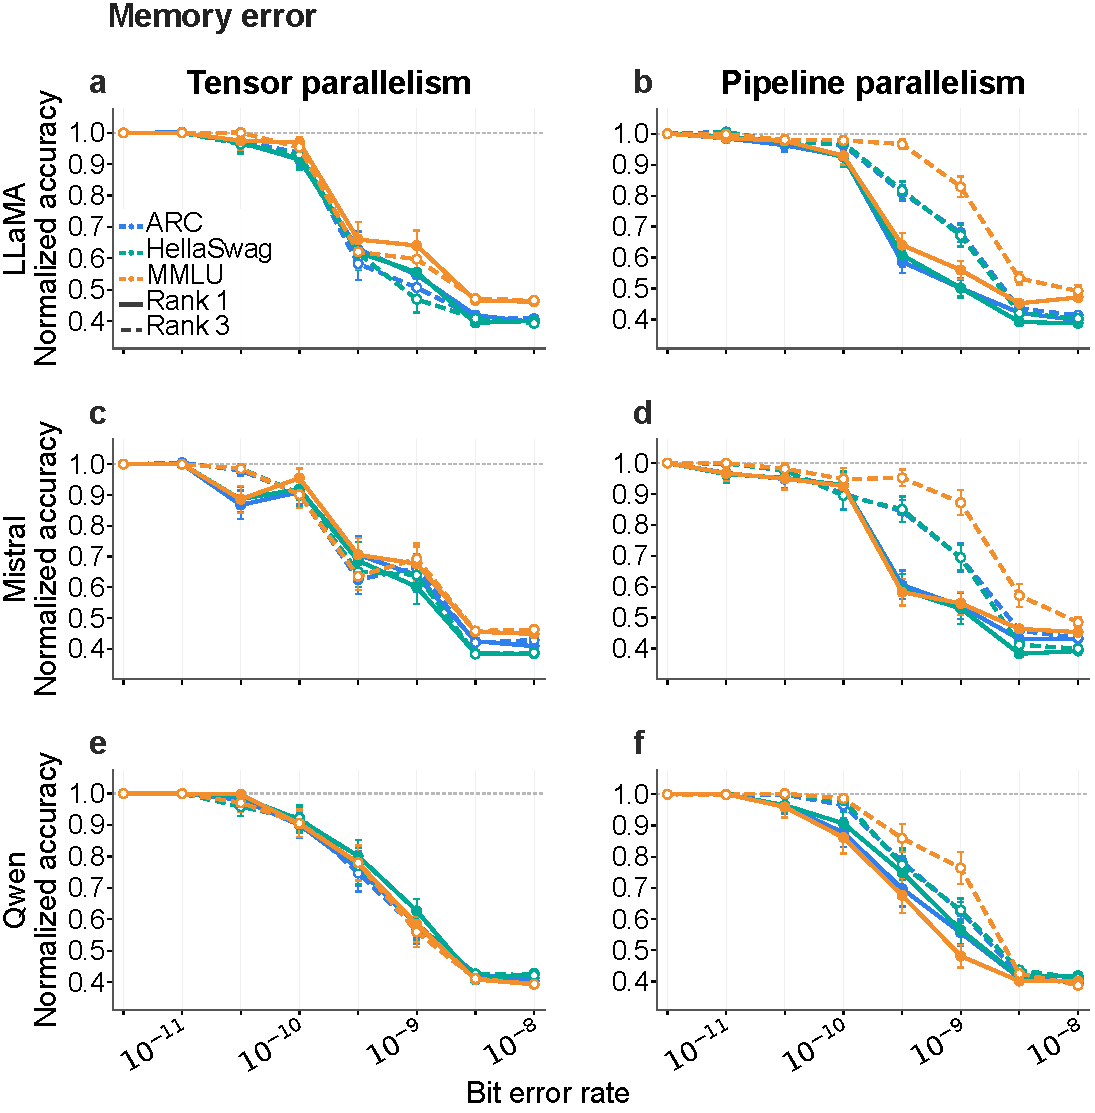
\includegraphics[width=\columnwidth]{fig_exp4_memory_compute_split_memory_error.pdf}
    \caption{\textbf{Rank and stage sensitivity under memory faults.}
    PP exhibits stronger position dependent vulnerability than TP.}
    \label{fig:parallel_memory_error}
\end{figure}

\begin{figure}[t]
    \centering
    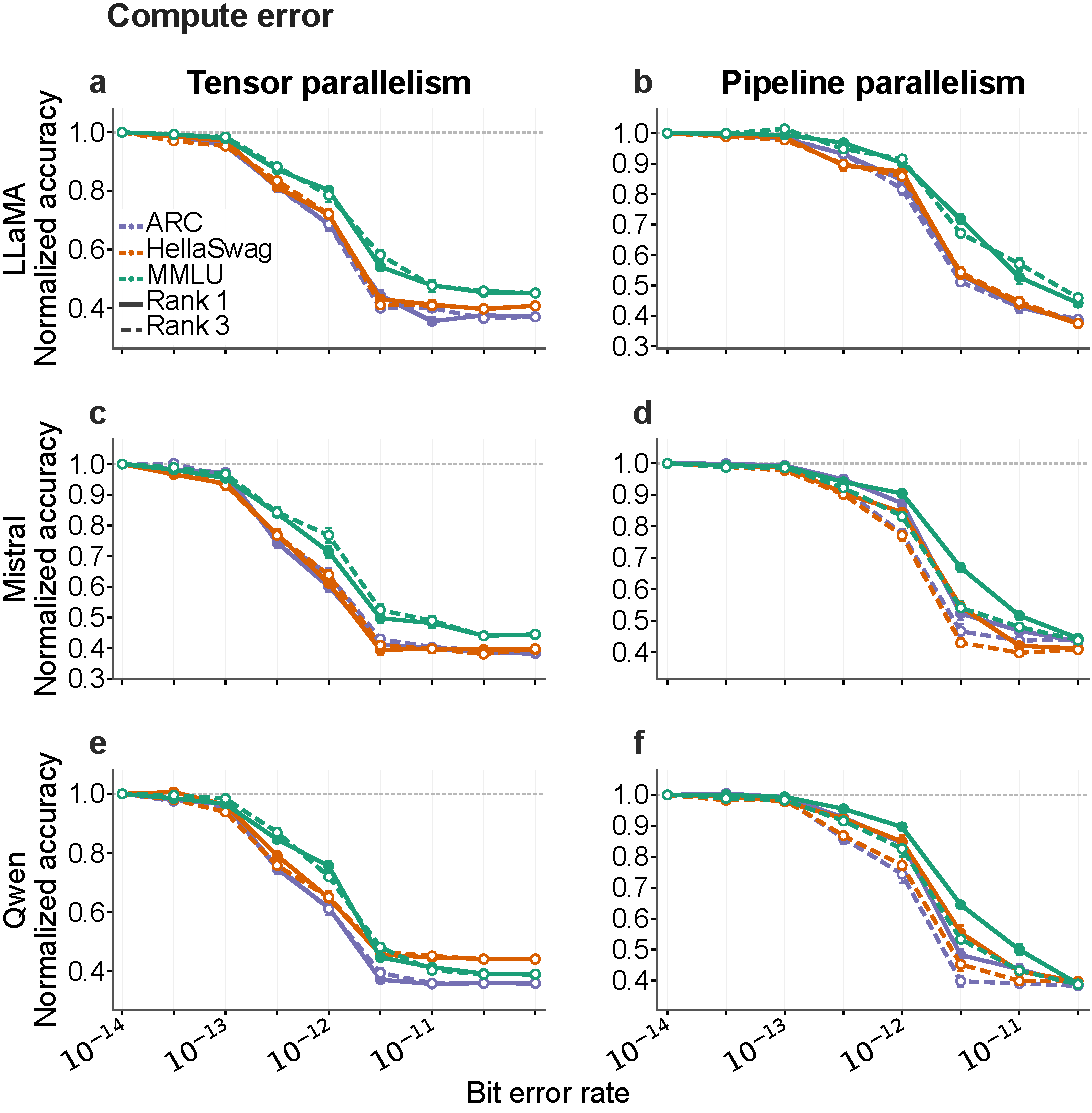
\includegraphics[width=\columnwidth]{fig_exp4_memory_compute_split_compute_error.pdf}
    \caption{\textbf{Rank and stage sensitivity under compute faults.}
    Later PP stages are more sensitive, while TP ranks show similar trends.}
    \label{fig:parallel_compute_error}
\end{figure}

As shown in Figures~\ref{fig:parallel_memory_error} and~\ref{fig:parallel_compute_error}, we evaluate LLaMA, Mistral, and Qwen under TP and PP configurations on ARC, HellaSwag, and MMLU. The parallel degree is fixed to 4. Fault-injection experiments are conducted separately on each of the four ranks. For each target rank, the injection scope covers all model layers or layer partitions assigned to that rank. Figures~10 and~11 report the results for Rank~1 and Rank~3, with the TP results shown in the left column and the PP results in the right column. This setup allows us to assess the effect of device position on model reliability.

\begin{observation}
\textbf{Observation 6:} Under TP, Rank 1 and Rank 3 show relatively similar degradation trends under both memory faults and compute faults. Under PP, reliability becomes more stage dependent: earlier stages are more sensitive to memory faults, whereas later stages show stronger sensitivity to compute faults.
\end{observation}

This difference is consistent with the partitioning structure of the two parallel strategies. TP partitions computation along tensor dimensions, so different ranks participate in the same layer computation with relatively symmetric roles. As a result, injecting faults into different TP ranks tends to produce similar degradation trends. In contrast, PP partitions the model along network depth, so different stages occupy different positions in the forward propagation path.

For memory faults, an error in an earlier PP stage corrupts the hidden state of a token earlier in the forward path. The perturbed representation is then propagated through more subsequent layers, increasing its chance to affect downstream representations and final predictions. In contrast, a memory fault in a later stage has a shorter propagation path before the output, which limits its opportunity to influence the model computation. For compute faults, the effect of an early local activation perturbation may be partially attenuated by later normalization, residual transformations, and layer wise computation. Faults injected into later PP stages are closer to the output and therefore have fewer subsequent layers in which their effects can be diluted, making them more directly visible in the final prediction.
